% status: 66
% chapter: TBD

\def\paperstatus{66} % a number from 0-100 indicating your status. 100
                % means completed
\def\paperchapter{TBD} % This section is typically a single keyword. from
                   % a small list. Consult with theinstructors about
                   % yours. They typically fill it out once your first
                   % text has been reviewed.
\def\hid{hid-sp18-705} % all hids of the authors of this
                                % paper. The paper must only be in one
                                % authors directory and all other
                                % authors contribute to it in that
                                % directory. That authors hid must be
                                % listed first
\def\volume{9} % the volume of the proceedings in which this paper is to
           % be included

\def\locator{\hid, Volume: \volume, Chapter: \paperchapter, 
	Status: \paperstatus. \newline}

\title{New Approaches to Managing Metadata at Scale in Research Libraries}
\author{Timothy A. Thompson}
\affiliation{%
  \institution{Indiana University Bloomington}
  \streetaddress{School of Informatics, Computing, and Engineering}
  \city{Bloomington} 
  \state{Indiana} 
  \postcode{47408}
}
\email{timathom@indiana.edu}

\begin{abstract} 
The analysis of big data often relies on distributed storage and
computation; however, access to big data---and to the platforms capable of
managing and processing it---continues to be largely centralized.
Centralization is particularly evident in the case of the metadata produced,
managed, and disseminated by academic and research libraries. Libraries
typically create and share their catalog records by uploading them to a
centrally managed database, which can then be searched by other libraries for
records that can be copied and added to an institution's local catalog. This
centralized approach, which operates on the basis of membership fees, has the
advantage of scalability and availability, but it comes at the cost of a loss
of autonomy. Although technical innovation is possible within the current
paradigm, the growing maturity of peer-to-peer protocols and decentralized
solutions points toward an alternative approach, one that would allow
libraries to share their data directly without having to pay an expensive
intermediary.
\end{abstract}

\keywords{i523, hid-sp18-705, Research Libraries, Library Catalogs, 
Peer-to-Peer, Blockchain}

\maketitle

\section{Introduction}
The problem of entity resolution (also known as record linkage or data
matching~\cite{pC12}) is one that has a direct impact on the work of
information professionals in research libraries. In library units
responsible for catalog management, many workflows center on a procedure
known as copy cataloging, which aims to expedite the processing of new
acquisitions. Copy cataloging involves searching a shared database for
records created by another cataloging agency, but that describe identical
publications that have been acquired by one's local institution~\cite{cD17}.
In the current environment, a single company, the Online Computer Library
Center (OCLC---\url{http://www.oclc.org}), is the only viable platform for
global cooperative cataloging~\cite{aT10}. OCLC provides data aggregation
and warehousing services that allow libraries to effectively share their
data, but its business model does not encourage peer-to-peer interaction and
innovation among individual libraries. This vendor-driven paradigm entails
the acceptance of a business model that, in effect, charges libraries for
serving their own data back to them, with some added value through quality
control and normalization. Once a library's data has been sent to OCLC, it
also becomes subject to potential licensing restrictions, as well as the
expectation that future dissemination of the data will include attribution
of OCLC~\cite{oclcND, oclc10}.

\section{New Approaches to Metadata Management}
Libraries have a tradition of experience with record matching and
automation~\cite{jM92}, but now stand to benefit from the increasingly
mainstream availability of algorithms and routines developed within the
context of data science and machine learning. Sophisticated algorithms for
string comparison and probabilistic record linkage have long been
available, but are not widely used by libraries, with the exception of
large-scale projects such as the Social Networks and Archival Context
Project (SNAC) (\url{http://snaccooperative.org/}) and the Virtual
International Authority File (VIAF) (\url{http://viaf.org/}). The former has
employed methods based on Naive Bayes classification algorithms to aggregate
and disambiguate data from across a wide range of libraries and archives
(the reported accuracy of the approach fell with the range of 80-90
percent)~\cite{rL11}. More recent approaches to record matching have
improved on probabilistic methods such as Naive Bayes by using Artificial
Neural Networks, improving accuracy rates in some cases to 98 percent or
more~\cite{rG17}.

As machine learning tools and methods have become more accessible,
however, large-scale, real-time access to library metadata has not
necessarily followed suit. The catalog of a large academic library may
contain around 10 million records~\cite{yul18}. By comparison, as of August
2018, the OCLC catalog database, WorldCat, contained 427,501,671
bibliographic records in 491 languages~\cite{oclc18}. As long as service
providers such as OCLC maintain centralized control over the aggregated
metadata of research libraries, large-scale computational analysis---and the
innovation it could produce---will remain proprietary and locked away.

New distributed technologies and protocols, including blockchains and
distributed hash tables (DHTs), could allow research libraries to form
robust peer-to-peer networks that would enable data sharing on a larger
scale. Although public blockchains such as Ethereum and Bitcoin are limited
in the amount of data that can feasibly be stored on chain, alternative
platforms that address this limitation have recently emerged. The
blockchain-based database service BigchainDB, implemented in Python,
provides a robust storage data solution while preserving the benefits of
blockchain features such as data immutability and an asset-based
transactional model. By running a consortial blockchain network of
BigchainDB nodes, libraries could be empowered to abandon centralized models
and begin managing their data collectively.

\section{Blockchains for Research Libraries}
Some in the library profession have been skeptical of blockchain
applications for their domain, arguing that blockchains are slow, expensive,
append-only databases that have been overhyped as a panacea~\cite{sjsu18}.
Even core developers of the Bitcoin blockchain have argued that the
constraints imposed by blockchain technology (such as immutability and
decentralized consensus) make it appropriate for a very limited set of
applications---namely, currency and the exchange of value~\cite{jSong18}.
For individuals and organizations who are investigating blockchains as a
technical solution, it is important from the outset to establish a framework
for evaluating their applicability and appropriateness~\cite{bS28}. For
example, a blockchain-based solution may be appropriate in a scenario in
which there is a lack of trust among participants, or in which processes and
collaboration would be more efficient if the need for trust were
eliminated~\cite{bS28}. In the case of a shared library catalog, trust is an
issue because not all participants can be trusted to provide data that
conforms to an expected level of quality. A commercial, centralized solution
mitigates these concerns by requiring participants to pay a membership fee.
A blockchain solution addresses issues of trust by enforcing a decentralized
consensus mechanism, which may take different forms, but which is designed
to ensure that participants can trust the network to maintain a consistent
state across all transactions~\cite{buchman2018latest}. 

The Proof-of-Stake consensus algorithm, employed by some blockchain
networks as an alternative to Bitcoin's resource-intensive Proof-of-Work
mechanism, is similar to the membership fee model in that validator nodes
are elected based on their share of ``stake'' in the network, measured by
their allocation of network tokens~\cite{gMarin18}. For research library
applications, a variation of Proof-of-Stake known as Proof-of-Authority may
be most appropiate~\cite{gMarin18, vButerin15}. In contrast to public
blockchains such as Ethereum and Bitcoin, or fully private blockchains
restricted to a single organization, so-called consortium blockchains may be
the preferred solution, one in which consensus ``is controlled by a
pre-selected set of nodes''~\cite{vButerin15}. The model implemented by the
BigchainDB project fits the parameters of a consortium
blockchain~\cite{bdb18b}.

\section{BigchainDB 2.0 Architecture}
\subsection{BigchainDB Server}


As of version 2.0, BigchainDB is Byzantine Fault Tolerant.

In BigchainDB 2.0, as is the case in general with systems that are
Byzantine fault tolerant, $3f + 1$ nodes are necessary to run a network,
where $f$ is the number of faulty nodes to be tolerated~\cite{bdb18}.
\subsection{Tendermint}
\subsection{MongoDB}






Shown in Figure~\ref{f:rbac}. 
Shown in Figure~\ref{f:bdb1}. 
Shown in Figure~\ref{f:bdb2}.


\begin{figure}[!htb]
	\centering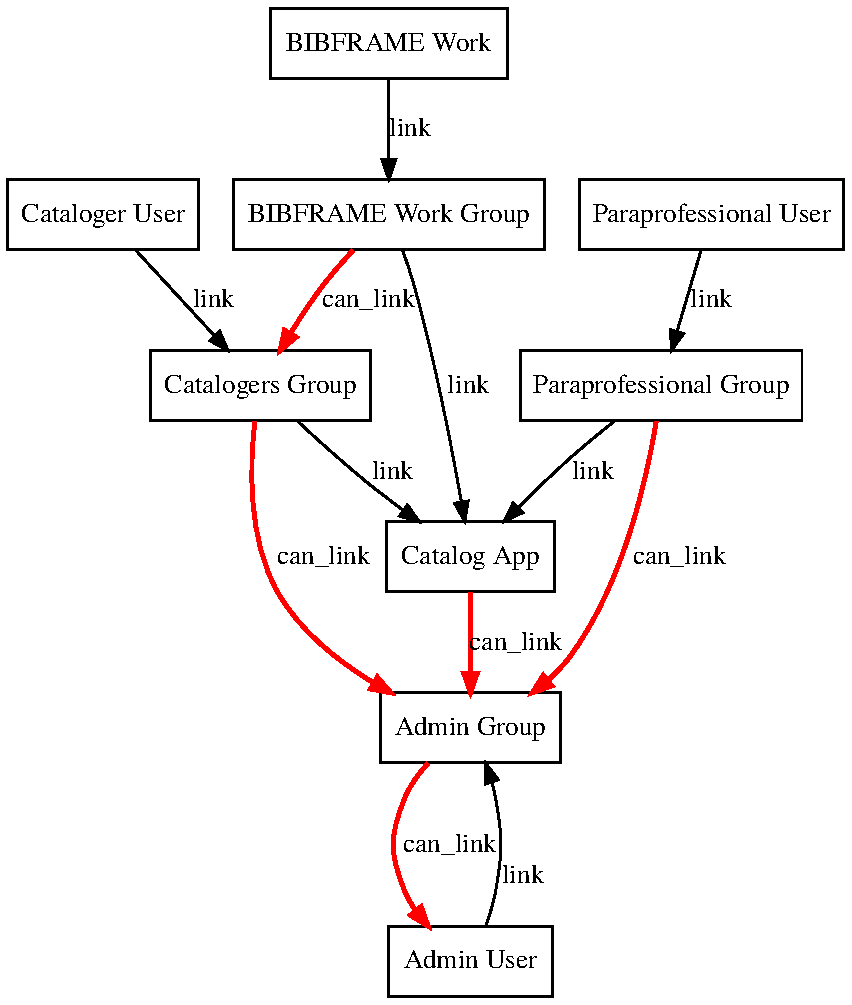
\includegraphics[width=\columnwidth]{images/rbac-graph.pdf}  
	\caption{Graph of permissions in BigchainDB using Role-Based Access 
	Control}\label{f:rbac}
\end{figure}

\begin{figure}[!htb]
	\centering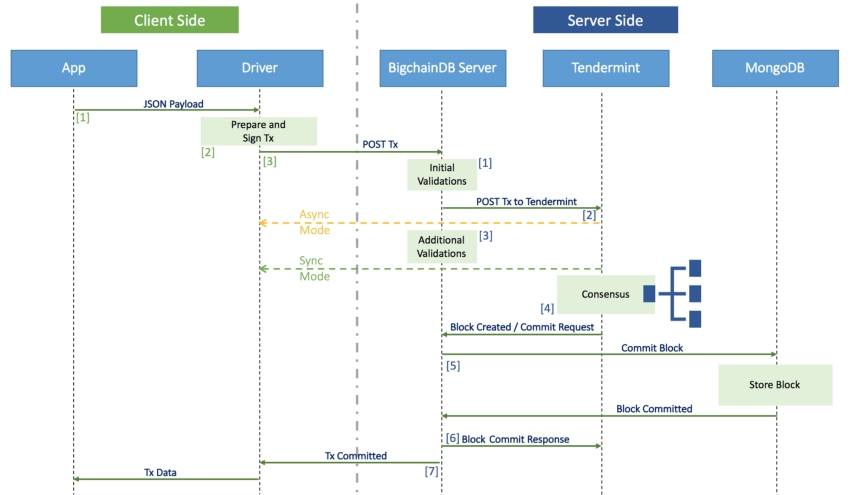
\includegraphics[width=\columnwidth]{images/bdb-seq.pdf}  
	\caption{BigchainDB Sequence Diagram~\cite{aA17}}\label{f:bdb1}
\end{figure}

\begin{figure}[!htb]
	\centering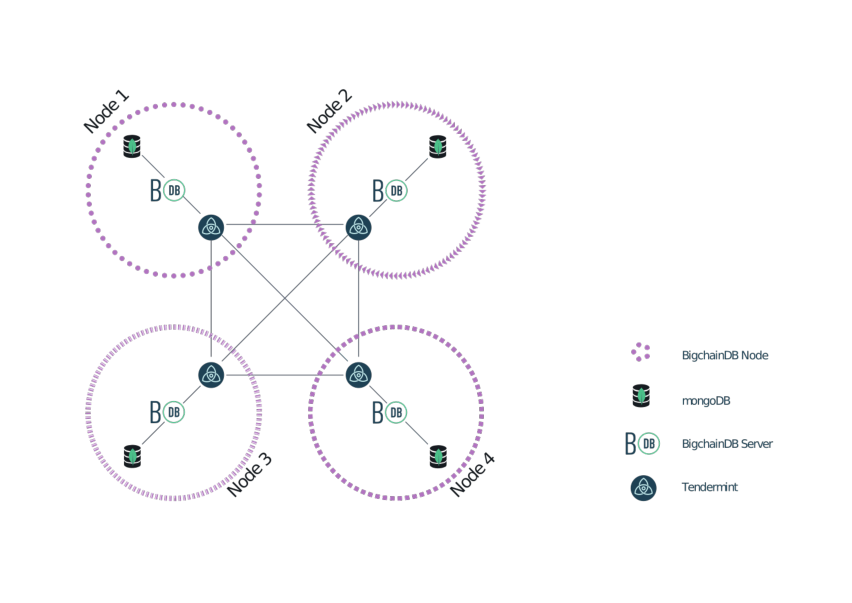
\includegraphics[width=\columnwidth]{images/bdb-arch.pdf}  
	\caption{BigchainDB Architecture Diagram~\cite{aA17}}\label{f:bdb2}
\end{figure}

\section{Conclusion}


\begin{acks}
The author would like to thank Dr.~Gregor~von~Laszewski and the i523
teaching assistants for their support and suggestions in writing this
report.
\end{acks}

\bibliographystyle{ACM-Reference-Format}
\bibliography{report} 

